\section{Architectural Overview}\label{sec:arch}

The basic architecture to develop a system like this, regarding the existing TUMOnline system where you can check if a student is enrolled or not, will consist of the following parts:

\begin{itemize}
\item The Smartphone, including a NFC Chip as well as an internet connection to register with the service. The internet connection will be needed only one time to initialize the system
\item The Door system, also including a NFC Chip which can send and receive. A NFC Reader would not be enough due to simple replay attacks. The Door system also needs access to the internet or at least to an intranet to check if the student or the employee has access to the specific area and to get other informations for realizing security features like communication encryption. Therefore, some kind of computer is also needed, interacting with the NFC hardware as well as with the backend.
\item A backend system, which will take care of key generation and storage in case of a public-key system.

\item The TUMOnline system since is in the possession of the enrollment information of every student.
\end{itemize} 
 
 A complete overview of the basic architecture: \newline
 \begin{center}
	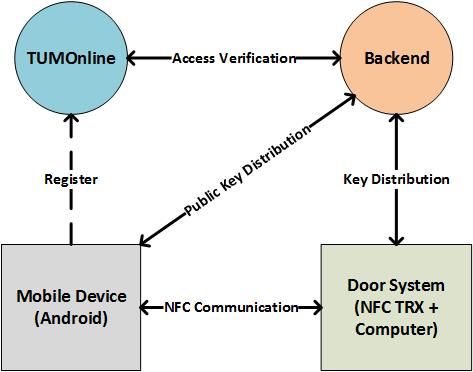
\includegraphics[scale=0.8]{basic_architecture.jpg}
\end{center}


\subsection{Registration with Backend}
To initialize the system, the user has to contact the backend system once for authentification. The connection is planned to be secured by HTTPS. The Backend system can check if the proposed login data of the user is valid or not. For that purpose, the connection to the TUMOnline service is needed to get this kind of  information. If the user has sent the right login combination, the backend system will create a public key pair and will send the user his private key. Therefore, a key storage and management system, a simple database has to be implemented.


\subsection{Authentication between Smartphone and NFC Transceiver}
After the user has registered with the backend system, he can communicate with the NFC Reader. As an initialization, there is a 3-Way-Handshake to provide a secure connection where the NFC Reader and the system behind will fetch the public key of the specific user. Further, the door system will check if the user has access to the requested area and will unlock the door depending on the outcome.

